\documentclass[UTF8,12pt,a4paper]{ctexart}

\usepackage[a4paper,left=2.6cm,right=2.6cm,top=2.5cm,bottom=2.5cm]{geometry}
\usepackage{amsmath,mathtools,amsthm}
\usepackage{unicode-math}
\setmathfont{STIX Math}
\setCJKmainfont{Noto Serif CJK SC}[BoldFont=Noto Serif CJK SC Bold]
\usepackage{booktabs,longtable,tabularx,array,multirow}
\usepackage{algorithm2e}
\usepackage{enumitem}
\usepackage{xcolor}
\usepackage{tikz}
\usetikzlibrary{positioning,arrows.meta,shapes.geometric}
\usepackage{hyperref}
\usepackage{cleveref}
\usepackage{microtype}
\usepackage{caption}
\usepackage{subcaption}
\usepackage{siunitx}
\usepackage{listings}

\hypersetup{
  colorlinks=true,
  linkcolor=black,
  citecolor=black,
  urlcolor=blue,
  pdftitle={一种离散时隙上的周期报文 Offset 均衡分配方法},
  pdfauthor={篠見由紀}
}

\pagestyle{plain}

\setlength{\parindent}{2em}
\setlength{\parskip}{0.25em}
\linespread{1.25}
\setlist[itemize]{leftmargin=2em,itemsep=0.25em,topsep=0.25em}
\setlist[enumerate]{leftmargin=2.5em,itemsep=0.25em,topsep=0.25em}

\newtheorem{definition}{定义}
\newtheorem{proposition}{命题}
\newtheorem{remark}{说明}

\DeclareMathOperator{\lcm}{lcm}
\DeclareMathOperator{\argmin}{arg\,min}
\DeclareMathOperator{\Var}{Var}
\newcommand{\ind}{\mathbb{I}}
\newcommand{\Oset}{\mathcal{A}}
\newcommand{\Rset}{\mathcal{R}}
\newcommand{\Sset}{\mathcal{S}}
\newcommand{\Mset}{\mathcal{M}}
\newcommand{\Hset}{\mathcal{H}}

\SetKwInput{KwInput}{输入}
\SetKwInput{KwOutput}{输出}
\SetKw{KwTo}{至}
\SetKw{KwAnd}{且}
\SetKw{KwBreak}{跳出}
\SetKwFunction{Evaluate}{Evaluate}
\SetKwFunction{Apply}{Apply}
\SetKwFunction{Remove}{Remove}
\SetKwFunction{Greedy}{GreedyConstruct}
\SetKwFunction{Local}{SingleRelocation}
\SetKwFunction{Pair}{ConflictPairSearch}

\lstset{
  basicstyle=\ttfamily\small,
  breaklines=true,
  frame=single,
  columns=fullflexible,
  showstringspaces=false
}

\title{\bfseries 一种离散时隙上的周期报文\\Offset 均衡分配方法}
\author{篠見由紀}
\date{2026年7月}

\begin{document}

\maketitle

\begin{abstract}
在汽车 CAN FD 网络中，多条周期报文若具有相同或高度聚集的首次发送延迟（Offset），其周期释放时刻会在超周期内反复重合，从而形成局部工作负载峰值。本文针对“仅调整周期报文初始 Offset，使报文释放在时间轴上尽量均匀”这一工程问题，建立离散时隙上的加权负载均衡模型。模型将 CAN FD 报文最坏传输时间作为负载权重，将 Offset 限定为有限离散集合，并以 5 ms 时隙峰值、超限程度、稳态离散度、启动阶段峰值和同时释放数量构成词典序目标。

在求解方法上，本文提出 GCLS（Greedy Construction and Conflict-directed Local Search）算法。该算法先依据周期和帧权重进行贪心构造，再通过单报文重定位、冲突导向双报文操作及随机重启改善解质量。为避免仅以启发式结果自证有效，本文同时给出原始配置、随机分配、纯贪心三类工程基线，并构建基于 CP-SAT 的整数优化模型作为小规模最优性对照。验证方案包括穷举校验、CP-SAT 最优性间隙、不同负载分布的重复实验、随机种子稳定性分析及 Vector/CANoe 结果对照。

本文以周期报文释放分布为直接研究对象，形成从启发式求解、精确对照到真实项目测量对照的完整验证闭环。所得结果用于评价 Offset 对局部峰值与整体均匀度的改善效果。
\end{abstract}

\noindent\textbf{关键词：} CAN FD；周期报文；Offset；负载均衡；贪心算法；局部搜索；CP-SAT

\tableofcontents
\newpage

\section{引言}

CAN 总线上的周期报文具有固定周期、固定发送节点和固定标识符。当多条报文采用相同的初始 Offset 时，它们会在启动时同时释放；若其周期具有公共倍数，则这种释放重合还会在后续运行中周期性重复。CAN 物理总线不能并行发送多帧，因此同时释放的报文最终表现为短时工作负载聚集、排队和局部高占用。

通过设置 Offset 对周期流量进行去同步化，已经是汽车 CAN 网络中常见的流量整形思路。已有研究指出，Offset 可以把工作负载摊开并降低峰值，从而改善报文响应时间，尤其是在总线负载较高时更为明显\cite{yomsi2012,grenier2008}。若项目目标是“通过初始 Offset 让周期报文尽量平均分布”，则可直接把每条 CAN FD 报文的传输时间作为释放事件权重，并在离散时隙上建立负载均衡模型。主问题可概括为：

\begin{quote}
给定一组周期 CAN FD 报文、每条报文的周期、传输时间权重以及可选 Offset 集合，为每条报文选择一个 Offset，使稳态超周期内的局部释放负载峰值最小，并在峰值相同的条件下使整体分布尽量均匀。
\end{quote}

本文的主要工作包括：

\begin{enumerate}
  \item 建立同时区分启动阶段与稳态阶段的离散时隙数学模型；
  \item 提出 GCLS 主算法，即“贪心构造 + 单报文重定位 + 冲突导向双报文搜索 + 随机重启”；
  \item 给出可重复的纯贪心、随机分配和原始配置基线；
  \item 构建 CP-SAT 整数模型，用于小规模实例的最优性对照；
  \item 设计从单元测试、穷举、精确求解到 Vector 工具对照的分层验证方法。
\end{enumerate}

\section{问题边界与基本假设}

\subsection{研究边界}

本文仅考虑 DBC 中定义的\textbf{周期 CAN FD 报文}，不考虑事件报文、诊断报文、网络管理报文及其他偶发流量。算法只计算推荐 Offset，不修改报文 ID、周期、DLC、发送节点和总线速率，也不负责回写 DBC 或 ARXML。

本文直接优化 Offset 所决定的报文释放时刻，以离散时隙内的加权释放负载描述局部聚集程度。该建模方式保持了问题边界清晰、目标可解释和求解规模可控。

\subsection{符号与输入}

设周期报文集合为
\begin{equation}
\Mset=\{m_1,m_2,\ldots,m_N\}.
\end{equation}

每条报文 $m_i$ 由下列参数描述：
\begin{equation}
 m_i=(T_i,C_i,O_i,\Oset_i),
\end{equation}
其中：

\begin{itemize}
  \item $T_i$：报文周期，单位为 ms；
  \item $C_i$：报文最坏总线占用时间，单位统一换算为 $\mu$s；
  \item $O_i$：待求的首次发送延迟；
  \item $\Oset_i$：报文允许选择的 Offset 集合。
\end{itemize}

当前工程约束为
\begin{equation}
\Oset_i=\{15,20,25,\ldots,100\}\ \mathrm{ms},\qquad \forall i.
\label{eq:offset-set}
\end{equation}

报文的第 $k$ 个实例释放时刻为
\begin{equation}
 r_{i,k}=O_i+kT_i,\qquad k=0,1,2,\ldots
\label{eq:release}
\end{equation}

\subsection{CAN FD 报文权重}

为避免把 8 字节帧与 64 字节帧简单视作相同负载，本文以最坏总线占用时间 $C_i$ 作为报文权重。若启用 BRS，则可抽象表示为
\begin{equation}
 C_i=\frac{N^{\mathrm{nom}}_i}{R_{\mathrm{nom}}}
     +\frac{N^{\mathrm{data}}_i}{R_{\mathrm{data}}},
\label{eq:frame-time-brs}
\end{equation}
其中 $N^{\mathrm{nom}}_i$ 和 $N^{\mathrm{data}}_i$ 分别为考虑最坏位填充后的仲裁相位与数据相位比特数；$R_{\mathrm{nom}}$、$R_{\mathrm{data}}$ 分别为 nominal bitrate 与 data bitrate。若未启用 BRS，则全帧按 nominal bitrate 计算：
\begin{equation}
 C_i=\frac{N^{\mathrm{nom}}_i+N^{\mathrm{data}}_i}{R_{\mathrm{nom}}}.
\label{eq:frame-time-no-brs}
\end{equation}

CAN FD 的帧格式、BRS 相位切换和 DLC 映射可依据 Bosch M\_CAN 文档实现\cite{boschmcan}。在算法层，$C_i$ 被视为已由独立帧时长计算模块得到的整数微秒值。

\subsection{平均负载可行性检查}

长期平均总线负载为
\begin{equation}
 U_{\mathrm{avg}}=\sum_{i=1}^{N}\frac{C_i}{T_i},
\label{eq:avg-load}
\end{equation}
其中 $C_i$ 与 $T_i$ 必须换算到相同时间单位。Offset 不改变单位时间内的发送次数，因此不会改变 $U_{\mathrm{avg}}$。

设项目平均负载上限为 $\beta=0.75$。若
\begin{equation}
 U_{\mathrm{avg}}>\beta,
\end{equation}
则仅靠 Offset 不可能把平均负载降到 75\%，算法应直接给出不可满足报告，而不是继续搜索。

\section{离散时隙负载模型}

\subsection{超周期与时隙}

定义周期集合的最小公倍数为
\begin{equation}
 H=\lcm(T_1,T_2,\ldots,T_N).
\label{eq:hyperperiod}
\end{equation}

当周期集合为 $\{10,20,50,100,500\}$ ms 时，$H=500$ ms。设时隙宽度为
\begin{equation}
 \Delta=5\ \mathrm{ms},
\end{equation}
则一个稳态超周期包含
\begin{equation}
 M=\frac{H}{\Delta}
\end{equation}
个时隙。对于上述周期集合，$M=100$。

\subsection{启动阶段与稳态阶段}

由于 Offset 是首次发送延迟，$O_i$ 与 $O_i+nT_i$ 在稳态下可能具有相同相位，但启动过程并不相同。为避免固定分析区间偏向更晚启动的报文，本文分别定义：

\begin{align}
 I^{\mathrm{st}}&=[0,O_{\max}),\\
 I^{\mathrm{ss}}&=[O_{\max},O_{\max}+H),
\end{align}
其中
\begin{equation}
 O_{\max}=\max_i\max \Oset_i.
\end{equation}

稳态区间长度固定为一个完整超周期，因此每条报文在 $I^{\mathrm{ss}}$ 内恰好释放 $H/T_i$ 次，与 Offset 的绝对大小无关；启动区间单独用于评价首次启动时的峰值。

定义报文 $i$ 在选择 Offset $o$ 时命中稳态时隙 $s$ 的指示量：
\begin{equation}
 a^{\mathrm{ss}}_{i,o,s}=
 \begin{cases}
 1, & \exists k:\ o+kT_i\in I^{\mathrm{ss}}_s,\\
 0, & \text{其他},
 \end{cases}
\label{eq:indicator-ss}
\end{equation}
其中 $I^{\mathrm{ss}}_s$ 表示稳态区间中的第 $s$ 个 5 ms 时隙。类似地定义启动阶段指示量 $a^{\mathrm{st}}_{i,o,s}$。

\subsection{时隙负载与释放计数}

给定 Offset 向量
\begin{equation}
 \symbf{O}=(O_1,O_2,\ldots,O_N),
\end{equation}
稳态时隙 $s$ 的加权负载为
\begin{equation}
 L^{\mathrm{ss}}_s(\symbf{O})=
 \sum_{i=1}^{N} C_i a^{\mathrm{ss}}_{i,O_i,s}.
\label{eq:slot-load}
\end{equation}

相应的同时释放报文数量为
\begin{equation}
 K^{\mathrm{ss}}_s(\symbf{O})=
 \sum_{i=1}^{N} a^{\mathrm{ss}}_{i,O_i,s}.
\label{eq:slot-count}
\end{equation}

启动阶段的 $L^{\mathrm{st}}_s$ 与 $K^{\mathrm{st}}_s$ 定义相同。

\subsection{5 ms 峰值约束}

将 5 ms 时隙内的释放工作量近似视为该窗口中的局部总线需求，则项目峰值约束为
\begin{equation}
 L^{\mathrm{ss}}_s(\symbf{O})\le B,
 \qquad B=\beta\Delta=0.75\times 5\ \mathrm{ms}=3.75\ \mathrm{ms}.
\label{eq:hard-constraint}
\end{equation}

当 $C_i$ 使用 $\mu$s 表示时，$B=3750\ \mu$s。本文以该约束衡量 5 ms 离散时隙内的加权释放负载，并在真实项目对照中同步统计 1 ms、5 ms 与 10 ms 窗口指标。

\section{优化目标}

\subsection{峰值与超限量}

定义稳态最大时隙负载：
\begin{equation}
 Z^{\mathrm{ss}}(\symbf{O})=\max_s L^{\mathrm{ss}}_s(\symbf{O}).
\label{eq:zss}
\end{equation}

定义启动阶段最大时隙负载：
\begin{equation}
 Z^{\mathrm{st}}(\symbf{O})=\max_s L^{\mathrm{st}}_s(\symbf{O}).
\label{eq:zst}
\end{equation}

若峰值硬约束暂时不可满足，则使用超限时隙数与总超限量衡量违反程度：
\begin{align}
 N_{\mathrm{vio}}(\symbf{O})
 &=\sum_s \ind\!\left[L^{\mathrm{ss}}_s(\symbf{O})>B\right],\\
 V_{\mathrm{vio}}(\symbf{O})
 &=\sum_s \max\left(0,L^{\mathrm{ss}}_s(\symbf{O})-B\right).
\label{eq:violations}
\end{align}

\subsection{均匀度指标}

稳态总工作量
\begin{equation}
 W=\sum_{s=1}^{M}L^{\mathrm{ss}}_s
\end{equation}
对任意 Offset 分配均为常数。平均时隙负载为
\begin{equation}
 \bar L=\frac{W}{M}.
\end{equation}

本文采用缩放后的绝对离差作为均匀度指标：
\begin{equation}
 D(\symbf{O})=
 \sum_{s=1}^{M}\left|M L^{\mathrm{ss}}_s(\symbf{O})-W\right|.
\label{eq:absolute-deviation}
\end{equation}

使用式\eqref{eq:absolute-deviation}而不直接使用浮点方差，有两个好处：一是保持整数运算；二是可直接在线性 CP-SAT 模型中通过辅助变量表达。

此外定义稳态最大同时释放数：
\begin{equation}
 K_{\max}(\symbf{O})=\max_s K^{\mathrm{ss}}_s(\symbf{O}).
\end{equation}

\subsection{词典序目标}

最终采用下列词典序目标向量：
\begin{equation}
 \symbf{F}(\symbf{O})=
 \left(
 N_{\mathrm{vio}},
 V_{\mathrm{vio}},
 Z^{\mathrm{ss}},
 Z^{\mathrm{st}},
 D,
 K_{\max}
 \right).
\label{eq:lexicographic-objective}
\end{equation}

两个解的优劣按照从左到右的顺序比较。也就是说：

\begin{enumerate}
  \item 优先减少违反 75\% 峰值约束的时隙数量；
  \item 再减少总超限量；
  \item 在可行解中优先降低稳态最大峰值；
  \item 再降低启动阶段峰值；
  \item 再使整体负载更加均匀；
  \item 最后减少同一时隙内的报文释放数量。
\end{enumerate}

词典序目标避免了人为设置加权系数。例如，使用简单加权和时，均匀度的改善可能错误地抵消峰值恶化；词典序目标不会出现这种情况。

\section{主算法：GCLS}

\subsection{总体结构}

GCLS 是 Greedy Construction and Conflict-directed Local Search 的缩写。算法流程如\cref{fig:gcls-flow}所示。

\begin{figure}[htbp]
\centering
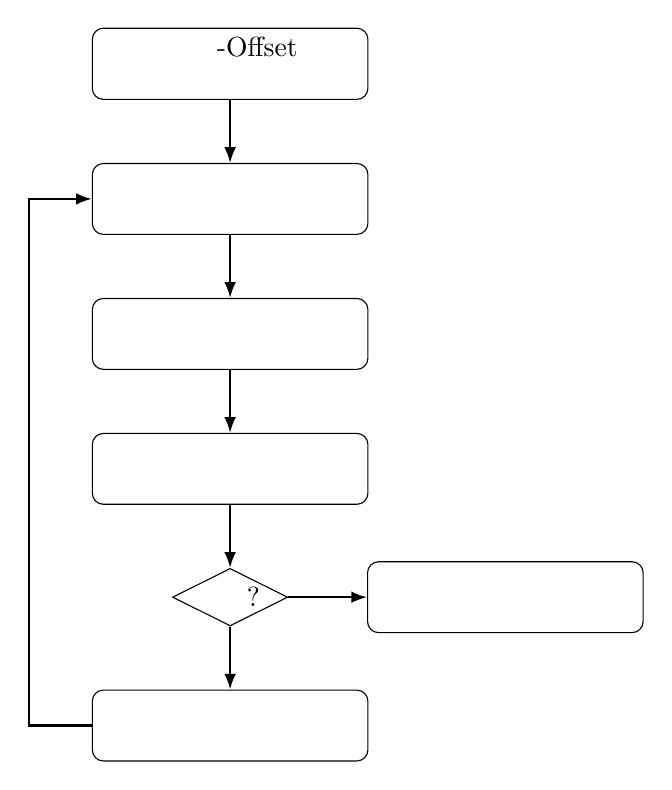
\begin{tikzpicture}[
  node distance=8mm and 10mm,
  box/.style={rectangle,draw,rounded corners,align=center,minimum width=3.5cm,minimum height=0.9cm},
  decision/.style={diamond,draw,aspect=2,align=center,inner sep=1pt},
  arrow/.style={-{Latex[length=2mm]},thick}
]
\node[box] (pre) {预计算所有报文-Offset\\命中时隙集合};
\node[box,below=of pre] (greedy) {贪心构造初始解};
\node[box,below=of greedy] (one) {单报文重定位搜索};
\node[box,below=of one] (pair) {冲突导向双报文搜索};
\node[decision,below=of pair] (restart) {达到重启次数?};
\node[box,right=of restart] (best) {保留全局最优解};
\node[box,below=of restart] (shuffle) {扰动同周期报文顺序\\重新构造};
\draw[arrow] (pre)--(greedy);
\draw[arrow] (greedy)--(one);
\draw[arrow] (one)--(pair);
\draw[arrow] (pair)--(restart);
\draw[arrow] (restart)--node[above]{是}(best);
\draw[arrow] (restart)--node[right]{否}(shuffle);
\draw[arrow] (shuffle.west) -| ([xshift=-8mm]greedy.west) |- (greedy.west);
\end{tikzpicture}
\caption{GCLS 算法流程}
\label{fig:gcls-flow}
\end{figure}

\subsection{候选时隙预计算}

对每条报文 $i$、每个候选 Offset $o\in\Oset_i$，预先计算命中稳态与启动时隙集合：
\begin{align}
 \Sset^{\mathrm{ss}}_{i,o}
 &=\{s\mid a^{\mathrm{ss}}_{i,o,s}=1\},\\
 \Sset^{\mathrm{st}}_{i,o}
 &=\{s\mid a^{\mathrm{st}}_{i,o,s}=1\}.
\end{align}

在试探某个候选 Offset 时，只需在相应集合中的时隙上加减 $C_i$，无需重新展开全部时间轴。

\subsection{贪心构造}

贪心阶段先按以下键值排序报文：
\begin{equation}
 \left(T_i,\ -C_i,\ \mathrm{ID}_i\right).
\label{eq:message-order}
\end{equation}
即周期越短越先处理；周期相同时，帧越长越先处理；仍相同时，以 CAN ID 保证确定性。短周期报文在超周期内出现次数更多，一旦位置选择不佳，对负载分布影响更大。

对每条报文，枚举全部候选 Offset，选择使当前部分解词典序目标最小的候选值。

\begin{algorithm}[htbp]
\caption{贪心构造算法}
\label{alg:greedy}
\KwInput{报文集合 $\Mset$，候选 Offset 集合 $\Oset_i$，预计算时隙集合}
\KwOutput{初始 Offset 向量 $\symbf{O}$}
按式\eqref{eq:message-order}对报文排序\;
初始化所有时隙负载为零\;
\ForEach{$m_i\in\Mset$}{
  $o^*\leftarrow \varnothing$，$F^*\leftarrow +\infty$\;
  \ForEach{$o\in\Oset_i$}{
    临时将 $m_i$ 以 Offset $o$ 加入当前状态\;
    $F\leftarrow \Evaluate(\symbf{O}\cup\{O_i=o\})$\;
    撤销临时加入\;
    \If{$F$ 按词典序优于 $F^*$}{
      $F^*\leftarrow F$，$o^*\leftarrow o$\;
    }
  }
  永久设置 $O_i\leftarrow o^*$ 并更新时隙状态\;
}
\Return{$\symbf{O}$}\;
\end{algorithm}

\subsection{单报文重定位局部搜索}

纯贪心的主要缺点是早期决策不可回退。单报文重定位（1-opt relocation）固定其他报文不变，依次重新枚举每条报文的所有候选 Offset。若新位置使全局目标改善，则接受移动。循环执行，直到完整一轮没有改进。

\begin{algorithm}[htbp]
\caption{单报文重定位局部搜索}
\label{alg:single-local}
\KwInput{贪心初始解 $\symbf{O}$}
\KwOutput{1-opt 局部最优解}
$improved\leftarrow true$\;
\While{$improved$}{
  $improved\leftarrow false$\;
  \ForEach{$m_i\in\Mset$}{
    保存当前 Offset $o_0\leftarrow O_i$\;
    从状态中移除 $m_i$\;
    在 $\Oset_i$ 中寻找使完整目标最优的 $o^*$\;
    将 $m_i$ 以 $o^*$ 重新加入状态\;
    \If{$o^*\neq o_0$ 且目标严格改善}{
       $O_i\leftarrow o^*$，$improved\leftarrow true$\;
    }
    \Else{
       恢复 $O_i\leftarrow o_0$\;
    }
  }
}
\Return{$\symbf{O}$}\;
\end{algorithm}

该阶段结束时，任意单条报文独立改变 Offset 都不能继续改善词典序目标，因此得到 1-opt 局部最优解。

\subsection{冲突导向双报文搜索}

1-opt 搜索可能停在平台区：任何单条报文移动都会先恶化目标，但两条报文同时移动却可能改善整体分布。为此，GCLS 只在最拥挤时隙附近进行有限的双报文搜索，而不枚举全部报文对。

设负载最高的前 $q$ 个稳态时隙集合为
\begin{equation}
 \Hset_q=\operatorname{TopQ}\left(\{L^{\mathrm{ss}}_s\}_{s=1}^{M}\right).
\end{equation}

定义冲突候选报文集合
\begin{equation}
 \mathcal{C}=\left\{m_i\mid \exists s\in\Hset_q,
 a^{\mathrm{ss}}_{i,O_i,s}=1\right\}.
\end{equation}

对 $\mathcal{C}$ 中的报文对 $(m_i,m_j)$，尝试两类操作：

\begin{enumerate}
  \item \textbf{双重定位：} $O_i$ 与 $O_j$ 同时移动到邻域候选；
  \item \textbf{Offset 交换：} 交换 $O_i$ 与 $O_j$，前提是交换后的值分别属于对方候选集合。
\end{enumerate}

邻域候选可限制为
\begin{equation}
 \mathcal{N}(O_i)=\{O_i\pm5,O_i\pm10,O_i\pm15\}\cap\Oset_i,
\end{equation}
以控制计算量。

\begin{algorithm}[htbp]
\caption{冲突导向双报文搜索}
\label{alg:pair-search}
\KwInput{当前 1-opt 解 $\symbf{O}$，热点时隙数 $q$，候选上限 $c$}
\KwOutput{改进后的 Offset 向量}
选择负载最高的 $q$ 个时隙，构造冲突报文集合 $\mathcal{C}$\;
按报文对热点负载的贡献排序，仅保留前 $c$ 条\;
\ForEach{$(m_i,m_j)\in \mathcal{C}\times\mathcal{C},\ i<j$}{
  \ForEach{$o_i\in\mathcal{N}(O_i)$}{
    \ForEach{$o_j\in\mathcal{N}(O_j)$}{
      试探双重定位 $(O_i,O_j)\leftarrow(o_i,o_j)$\;
      \If{目标严格改善}{接受并重新执行单报文局部搜索\;}
    }
  }
  \If{交换 $O_i,O_j$ 合法且目标严格改善}{接受交换并重新执行单报文局部搜索\;}
}
\Return{$\symbf{O}$}\;
\end{algorithm}

\subsection{随机重启}

贪心构造对报文排序敏感。为了降低这一敏感性，执行 $K$ 次随机重启。每次重启保持“周期升序、权重降序”的大类顺序，仅对周期相同且权重接近的报文随机打乱。每次运行完整的“贪心 + 1-opt + 冲突双报文”流程，并保留全局最优结果。

随机重启不是通过随机接受劣解来跳出局部最优，因此比模拟退火更容易复现和解释。本文默认取 $K=20$，并记录全部随机种子。

\section{对照算法}

\subsection{原始 Offset 配置}

若项目 DBC 中已有 Offset，则直接以原始配置作为工程基线：
\begin{equation}
 \symbf{O}^{\mathrm{orig}}.
\end{equation}

若原始项目全部为 0，但 0 不属于新候选集合，则原始配置只用于展示优化前释放聚集，不作为约束内可行解。

\subsection{随机分配}

对每条报文独立均匀采样：
\begin{equation}
 O_i\sim \operatorname{Uniform}(\Oset_i).
\end{equation}

重复 $R$ 次，报告目标指标的中位数、最好值和最差值。随机分配用于衡量“随便错开”能达到的水平，并检验 GCLS 的改进是否来自算法本身，而不是仅仅来自 Offset 非零。

\subsection{纯贪心}

纯贪心采用\cref{alg:greedy}，不执行局部搜索。它是最重要的消融基线，用于量化局部求解器带来的收益：
\begin{equation}
 \Delta Z=Z_{\mathrm{greedy}}-Z_{\mathrm{GCLS}}.
\end{equation}

若 $\Delta Z=0$，仍需比较均匀度 $D$、热点时隙数量及启动峰值。

\subsection{CP-SAT 精确对照}

CP-SAT 适合处理离散整数决策，可返回 OPTIMAL、FEASIBLE、INFEASIBLE 或 UNKNOWN 等求解状态\cite{ortools}. 本文用其建立小规模精确或限时近似最优基线。

对每条报文 $i$ 和候选 Offset $o\in\Oset_i$，定义二元变量
\begin{equation}
 x_{i,o}=\begin{cases}
 1,& O_i=o,\\
 0,& \text{其他}.
 \end{cases}
\end{equation}

唯一选择约束为
\begin{equation}
 \sum_{o\in\Oset_i}x_{i,o}=1,
 \qquad \forall i.
\label{eq:cp-one}
\end{equation}

稳态时隙负载为
\begin{equation}
 L_s=\sum_{i=1}^{N}\sum_{o\in\Oset_i}
 C_i a^{\mathrm{ss}}_{i,o,s}x_{i,o}.
\label{eq:cp-load}
\end{equation}

引入最大负载变量 $Z$：
\begin{equation}
 L_s\le Z,\qquad \forall s.
\label{eq:cp-z}
\end{equation}

若要求验证 75\% 峰值可行性，再加入
\begin{equation}
 L_s\le B,\qquad \forall s.
\label{eq:cp-hard}
\end{equation}

为表达绝对离差，引入非负整数变量 $d_s$：
\begin{align}
 d_s&\ge M L_s-W,\\
 d_s&\ge W-M L_s,
\end{align}
并定义
\begin{equation}
 D=\sum_s d_s.
\end{equation}

最大释放数量可由
\begin{align}
 K_s&=\sum_i\sum_o a^{\mathrm{ss}}_{i,o,s}x_{i,o},\\
 K_s&\le K_{\max}
\end{align}
表示。

为了保持词典序，与其构造一个巨大加权和，更稳妥的方式是分阶段求解：

\begin{enumerate}
  \item 最小化 $Z$，得到 $Z^*$；
  \item 加入 $Z=Z^*$，最小化 $D$，得到 $D^*$；
  \item 加入 $D=D^*$，最小化 $K_{\max}$；
  \item 如需考虑启动峰值，可进一步固定前三阶段结果并最小化 $Z^{\mathrm{st}}$。
\end{enumerate}

若硬约束模型不可行，则移除式\eqref{eq:cp-hard}，最小化 $Z$，求得当前网络在给定 Offset 集合下能达到的理论最低稳态峰值。

\section{复杂度分析}

设：

\begin{itemize}
  \item $N$：报文数量；
  \item $A=|\Oset_i|$：每条报文候选 Offset 数，当前为 18；
  \item $M=H/\Delta$：稳态时隙数量，当前典型值为 100；
  \item $r_i=H/T_i$：报文 $i$ 在一个稳态超周期内的释放次数；
  \item $K$：随机重启次数；
  \item $I$：单报文局部搜索迭代轮数。
\end{itemize}

预计算命中时隙集合的复杂度为
\begin{equation}
 O\left(\sum_{i=1}^{N}A r_i\right).
\end{equation}

若每次候选评估对所有 $M$ 个时隙重新扫描，贪心构造复杂度为
\begin{equation}
 O(NAM).
\end{equation}

利用命中集合增量更新后，试探性加减负载的代价近似为 $O(r_i)$；由于当前 $M=100$ 很小，评分阶段保留 $O(M)$ 全扫描更利于保证代码正确性。

单报文局部搜索每轮复杂度同样为
\begin{equation}
 O(NAM),
\end{equation}
总复杂度约为 $O(INAM)$。

设冲突候选集合上限为 $c$，每条报文邻域候选数量为 $b$，则双报文搜索最坏复杂度为
\begin{equation}
 O(c^2b^2M).
\end{equation}

GCLS 总体复杂度近似为
\begin{equation}
 O\left(K\left[(I+1)NAM+c^2b^2M\right]\right).
\end{equation}

在 $N\approx20$、$A=18$、$M=100$、$K\le30$ 的项目规模下，该计算量对 Python 实现通常很轻。CP-SAT 的最坏复杂度仍具有组合爆炸风险，因此其定位是小规模对照和限时验证，而不是唯一工程主算法。

\section{正确性与不变量}

虽然 GCLS 不能保证全局最优，但实现必须满足以下基本不变量。

\begin{proposition}[Offset 合法性]
算法输出满足
\begin{equation}
 O_i\in\Oset_i,\qquad \forall i.
\end{equation}
\end{proposition}

\begin{proposition}[稳态释放次数守恒]
在区间 $I^{\mathrm{ss}}=[O_{\max},O_{\max}+H)$ 内，每条报文 $i$ 的释放次数恒为 $H/T_i$，与 $O_i$ 无关。
\end{proposition}

\begin{proof}
区间长度为 $H$，且 $H$ 是 $T_i$ 的整数倍。周期序列 $O_i+kT_i$ 在任意长度为 $H$ 的半开区间内恰好出现 $H/T_i$ 个元素。
\end{proof}

\begin{proposition}[稳态总负载守恒]
对于任意合法 Offset 向量 $\symbf{O}$，有
\begin{equation}
 \sum_{s=1}^{M}L^{\mathrm{ss}}_s(\symbf{O})
 =\sum_{i=1}^{N}\frac{H}{T_i}C_i=W.
\end{equation}
\end{proposition}

该性质用于单元测试：任何 apply/rollback、局部移动或双报文操作后，稳态总负载都不得改变。

\begin{proposition}[局部搜索单调性]
若局部搜索只接受严格改善词典序目标的操作，则算法产生的目标序列严格下降，并将在有限步内停止。
\end{proposition}

\begin{proof}
合法 Offset 组合数量为有限值 $\prod_i|\Oset_i|$。每次接受操作都使词典序目标严格下降，因此不会重复访问同一目标状态，也不可能无限执行。
\end{proof}

\section{实验设计与验证方法}

\subsection{对照组}

本文设置表\ref{tab:baselines}所示的五组对照方法。

\begin{table}[htbp]
\centering
\caption{算法对照组}
\label{tab:baselines}
\begin{tabularx}{\textwidth}{lXl}
\toprule
方法 & 作用 & 结果性质\\
\midrule
Original & 原始 Vector/DBC Offset 配置 & 工程现状基线\\
Random & 独立随机选择 Offset，多次重复 & 随机错峰基线\\
Greedy & 仅运行贪心构造 & 消融局部搜索收益\\
GCLS & 贪心 + 1-opt + 冲突双报文 + 重启 & 主工程算法\\
CP-SAT & 整数约束优化，限时或求最优 & 小规模最优性对照\\
\bottomrule
\end{tabularx}
\end{table}

\subsection{主要评价指标}

定义 5 ms 稳态峰值负载率：
\begin{equation}
 P_5=\frac{Z^{\mathrm{ss}}}{\Delta}.
\end{equation}

启动峰值负载率：
\begin{equation}
 P^{\mathrm{st}}_5=\frac{Z^{\mathrm{st}}}{\Delta}.
\end{equation}

均匀度可使用归一化绝对离差：
\begin{equation}
 D_{\mathrm{norm}}=
 \frac{1}{MW}\sum_s\left|ML_s-W\right|.
\end{equation}

也可报告变异系数：
\begin{equation}
 \mathrm{CV}=\frac{\sqrt{\frac{1}{M}\sum_s(L_s-\bar L)^2}}{\bar L}.
\end{equation}

相对于原始配置的峰值改善率：
\begin{equation}
 \eta_Z=\frac{Z_{\mathrm{orig}}-Z_{\mathrm{alg}}}{Z_{\mathrm{orig}}}\times100\%.
\end{equation}

当 CP-SAT 求得最优峰值 $Z^*$ 时，GCLS 的最优性间隙为
\begin{equation}
 \mathrm{Gap}_Z=
 \frac{Z_{\mathrm{GCLS}}-Z^*}{\max(Z^*,1)}\times100\%.
\end{equation}

若 CP-SAT 只在时限内得到下界 $LB$，则报告
\begin{equation}
 \mathrm{Gap}_{LB}=
 \frac{Z_{\mathrm{GCLS}}-LB}{\max(LB,1)}\times100\%.
\end{equation}

本文同时报告：

\begin{itemize}
  \item 超限时隙数 $N_{\mathrm{vio}}$ 与总超限量 $V_{\mathrm{vio}}$；
  \item 最大同时释放报文数 $K_{\max}$；
  \item 算法运行时间；
  \item GCLS 多个随机种子下的均值、标准差、最好值与最差值；
  \item 局部搜索相对于纯贪心的增量改善。
\end{itemize}

\subsection{验证层次}

\subsubsection{单元级数学一致性}

必须验证：

\begin{enumerate}
  \item 预计算时隙集合与直接展开释放时刻的结果完全一致；
  \item 增量 apply/rollback 后，全部负载数组和目标值恢复原状；
  \item 稳态总释放次数和总负载满足守恒命题；
  \item 所有输出 Offset 均属于合法集合；
  \item 局部搜索接受操作后，词典序目标严格改善。
\end{enumerate}

\subsubsection{穷举验证}

对于小规模实例，直接枚举所有 Offset 组合：
\begin{equation}
 |\Omega|=A^N.
\end{equation}

当 $A=18$ 时，本文对 $N\le5$ 的实例执行完整穷举；对于 $N\le8$ 的实例，通过缩小候选 Offset 集合执行补充穷举。穷举结果用于确认：

\begin{itemize}
  \item CP-SAT 模型与直接评价函数的一致性；
  \item GCLS 是否能找到全局最优或接近最优解；
  \item 词典序比较实现是否正确。
\end{itemize}

\subsubsection{CP-SAT 对照}

对 8--20 条报文的小中规模实例设置固定求解时限，例如 60 s 或 300 s。报告求解状态、最优目标、最佳下界和时限内 gap。若 CP-SAT 返回 OPTIMAL，则可直接评价 GCLS 的真实最优性间隙；若返回 FEASIBLE，则仅以其下界和当前最好解进行夹逼。

\subsubsection{真实项目对照}

将 GCLS 输出的 Offset 手动配置到 Vector 工具或等价仿真环境中，对比：

\begin{itemize}
  \item 报文释放时刻图；
  \item 1 ms、5 ms、10 ms 滑动窗口真实总线占用率；
  \item 最大连续忙碌时间；
  \item 优化前后热点时间点及峰值位置的一致性；
  \item 离散模型与实测窗口负载的相对误差。
\end{itemize}

该对照用于量化离散释放负载模型与真实 CAN FD 项目测量结果之间的一致性及误差范围。

\subsection{测试集设计}

\begin{table}[htbp]
\centering
\caption{实验数据集}
\label{tab:testsets}
\begin{tabularx}{\textwidth}{lclX}
\toprule
数据集 & 报文数 & 周期特征 & 验证目标\\
\midrule
四报文示例 & 4 & 10/20/50/100 ms & 人工核对释放时刻与最优 Offset\\
小规模均衡集 & 6--8 & 周期较均匀 & 穷举与 CP-SAT 精确对照\\
高频拥挤集 & 12 & 10/20 ms 较多 & 检验峰值约束与冲突搜索\\
典型混合集 & 20 & 100 ms 最多，10 ms 最少 & 主工程性能评价\\
大帧压力集 & 20 & 48/64 B 报文较多 & 检验加权模型优于报文计数\\
扩展集 & 50--100 & 保持典型周期集合 & 运行时间与稳定性分析\\
\bottomrule
\end{tabularx}
\end{table}

\section{示例说明}

考虑四条周期报文，周期分别为
\begin{equation}
 (T_1,T_2,T_3,T_4)=(20,100,10,50)\ \mathrm{ms}.
\end{equation}

若四条报文均以 $O_i=0$ 启动，则在 $t=0,100,200,\ldots$ ms 时四条报文同时释放。若所有帧权重相等，则这些时隙的释放计数为 4，其余部分时隙负载较低。

GCLS 会先处理 10 ms 周期报文，再处理 20 ms、50 ms 和 100 ms 报文。假设候选集合为式\eqref{eq:offset-set}，算法可能得到类似
\begin{equation}
 (O_1,O_2,O_3,O_4)=(20,35,15,25)\ \mathrm{ms}
\end{equation}
的候选解。该示例数值仅用于说明形式，最终结果必须由实际 $C_i$、Offset 候选和词典序目标计算得到。

需要特别注意：对于 10 ms 周期报文，15 ms 与 25 ms 在稳态具有相同相位，但启动时刻不同。因此本文把稳态分布作为主优化对象，同时保留启动峰值作为次级目标。

\section{实现方法}

数学求解模块仅依赖统一数据模型，不直接读取 DBC 或 ARXML。输入层完成文件解析后，向优化器提供：

\begin{lstlisting}
Message(
    name,
    cycle_time_us,
    frame_time_us,
    allowed_offsets_us,
    original_offset_us,
    sender_ecu,
)
\end{lstlisting}

核心优化器只需维护：

\begin{itemize}
  \item \texttt{steady\_slot\_loads[s]}；
  \item \texttt{startup\_slot\_loads[s]}；
  \item \texttt{steady\_slot\_counts[s]}；
  \item 每个 $(i,o)$ 的稳态/启动命中时隙集合；
  \item 当前 Offset 向量与词典序目标。
\end{itemize}

本文将主算法、对照算法与验证模块组织为：

\begin{lstlisting}
optimizers/
  greedy.py
  local_search.py
  gcls.py
  cp_sat.py

evaluation/
  metrics.py
  objective.py
  exhaustive.py
\end{lstlisting}

其中 \texttt{gcls.py} 构成默认求解流程，\texttt{cp\_sat.py} 和 \texttt{exhaustive.py} 用于精确对照与回归测试。

\section{适用范围与结果解释}

本文模型优化的是周期报文释放工作量在离散时间轴上的分布。其评价结果直接反映 Offset 对峰值时隙、超限时隙数量、整体离散度、启动峰值及同时释放数量的影响。

模型的适用范围限定如下：

\begin{enumerate}
  \item 5 ms 时隙模型描述时隙尺度上的释放负载，不刻画帧在时隙内部的精确连续位置；
  \item 研究对象限于 DBC 中定义的周期 CAN FD 报文，不包含偶发流量、发送抖动、时钟漂移及错误重传；
  \item 75\% 为本项目采用的设计阈值，用于判定 5 ms 时隙负载是否满足工程约束；
  \item 算法结论以 Offset 均衡分配效果为边界，不将离散负载指标外推为完整的端到端时延证明。
\end{enumerate}

本文通过数学一致性测试、穷举、CP-SAT 对照和 Vector/CANoe 项目测量共同验证结论。四类验证使用同一 Offset 向量与统一评价口径，从而保证算法结果、精确模型和工程观测之间具有可比性。

\section{结论}

本文针对 CAN FD 周期报文初始 Offset 均衡分配问题，建立了边界明确的离散时隙优化模型，直接解决报文释放时刻错开与超周期局部负载均衡问题。

GCLS 以贪心构造提供高质量初始解，通过单报文重定位消除早期贪心决策的局限，再利用冲突导向双报文操作突破 1-opt 平台，并通过随机重启降低排序敏感性。纯贪心、随机分配与原始配置构成工程对照，CP-SAT 和穷举则提供小规模最优性验证。该组合兼顾可解释性、实现难度、运行速度和学术验证完整性，适合约 20 条乃至更大规模的典型周期报文集合。

\begin{thebibliography}{99}

\bibitem{yomsi2012}
P. M. Yomsi, D. Bertrand, N. Navet, and R. I. Davis.
Controller Area Network (CAN): Response Time Analysis with Offsets.
In \emph{Proceedings of the IEEE International Workshop on Factory Communication Systems (WFCS)}, 2012.

\bibitem{grenier2008}
M. Grenier, L. Havet, and N. Navet.
Pushing the Limits of CAN---Scheduling Frames with Offsets Provides a Major Performance Boost.
In \emph{Proceedings of the 4th European Congress Embedded Real Time Software}, 2008.

\bibitem{tindell1994}
K. Tindell, H. Hansson, and A. Wellings.
Analyzing Real-Time Communications: Controller Area Network (CAN).
In \emph{Proceedings of the 15th IEEE Real-Time Systems Symposium (RTSS)}, 1994.

\bibitem{boschmcan}
Robert Bosch GmbH.
\emph{M\_CAN User's Manual}, Revision 3.3.1.
Available at: \url{https://www.bosch-semiconductors.com/media/ip_modules/pdf_2/m_can/mcan_users_manual_v331.pdf}.

\bibitem{ortools}
Google Optimization Team.
\emph{CP-SAT Solver, OR-Tools Documentation}.
Available at: \url{https://developers.google.com/optimization/cp/cp_solver}, accessed July 2026.

\end{thebibliography}

\end{document}
